\subsection{Introducción:}

En este ejercicio realizaremos el \textit{scheduler}.

\begin{itemize}

\item [\textit{a)}]  Construir una función para inicializar las estructuras de datos del \textit{scheduler}.

\item [\textit{b)}] Crear la función  \textit{sched\_proxima\_a\_ejecutar()} que devuelve el  índice de la próxima tarea a ser ejecutada. 

\item [\textit{c)}]  Crear una función \textit{sched\_atender\_tick()} que llame a \textit{game\_atender\_tick()} pasando el número de tarea actual y luego devuelva el índice en la gdt al cual se deberá saltar. Reemplazar el llamado a \textit{game\_atender\_tick} por uno a \textit{sched\_atender\_tick} en el handler de la interrupción de reloj.

\item [\textit{d)}] Modificar la rutina de la interrupción 0x46, para que implemente los servicios según se indica en la sección 4.4.13

\item [\textit{e)}]  Modificar el código necesario para que se realice el intercambio de tareas por cada ciclo de reloj. El intercambio se realizará a según indique la función \textit{sched\_proxima\_a\_ejecutar().}

\item [\textit{f)}]  Modificar las rutinas de excepciones del procesador para que desalojen a la tarea que estaba corriendo y corran la próxima.

\item [\textit{g)}] Implementar el mecanismo de debugging explicado en la sección 4.8 que indicará en pantalla la razón del desalojo de una tarea.

\end{itemize}

\subsection{Ítem a): Inicializar el \textit{scheduler}}

Para incializar el scheduler completamos la funicón \textit{void sched\_inicializar()} del archivo sched.d. En el tp el scheduler es una estructura que posee un array de tareas denimoinado \textit{tasks} y un int denominado \textit{current} en el cual se guarda la tarea actual. Las tareas tambien son estructuras, y contienen un int para recordar la posicion en la que se guarda en la gdt y un puntero a la tarea que representan. Esta estructura se puede obserbar en la siguiente imagen:

\begin{figure}[H]
\begin{center}
\minipage{0.5\textwidth}
 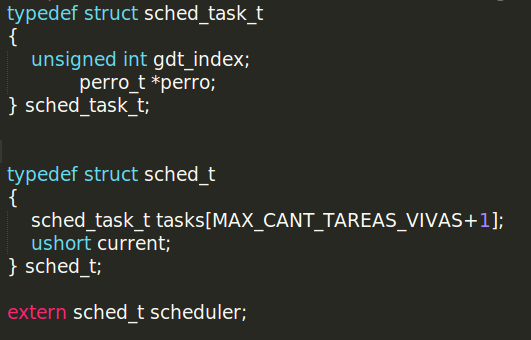
\includegraphics[width=\linewidth]{ejercicio7/sched.png}
 \caption{{\small Estrctura del scheduler usado} }
\endminipage
\end{center}
\end{figure}

La función en cuestión es la siguiente:

\begin{figure}[H]
\begin{center}
\minipage{0.5\textwidth}
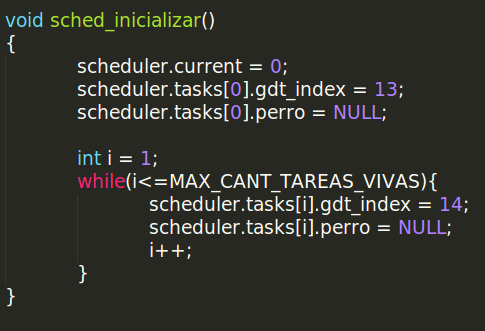
\includegraphics[width=\linewidth]{ejercicio7/funcion.png}
\caption{{\small \textit{void sched\_inicializar()} }}
\endminipage
\end{center}
\end{figure}

Para inicializar la estructura del scheduler realiza lo siguiente:

\begin{itemize}

\item [\textit{A}] Setea el valor de \textit{current} en 0, pues la tarea inicial debe ser la tarea \textit{IDLE} y por convención decidimos que esta se encuentre en la posición 0 del array de tareas. Devido a la decisión anterior, setiamos en el vector de tareas que el gdt\_index de la tarea 0 sea 13 (posición en la \textit{GDT} de la tarea \textit{IDLE} ) y que el puntero a la tarea de la tarea 0 sea \textit{NULL}.

\item [\textit{B}] Luego itera por todo el array de tareas \textit{tasks} seteandole a cada tarea una posición en la gdt correspondiente y seteando el puntero decada una en \textit{NULL}.

\end{itemize}

\subsection{Ítem b):  Crear la función  \textit{sched\_proxima\_a\_ejecutar()}}

Esta función comienza guardando cual es el jugador de la tarea actual y busca las siguiente tarea que corresponda al suiguiente jugador. Para esto itera por todas las tareas y se fija entre las que no tienen un puntero a una tarea \textit{NULL} si alguna pertence al jugador contrario, en caso de que no la encuentre busca devuelta entre todas las tareas pero solo fijandose si no tienen un puntero a una tarea  \textit{NULL}.

\begin{figure}[H]
\begin{center}
\minipage{1.00\textwidth}
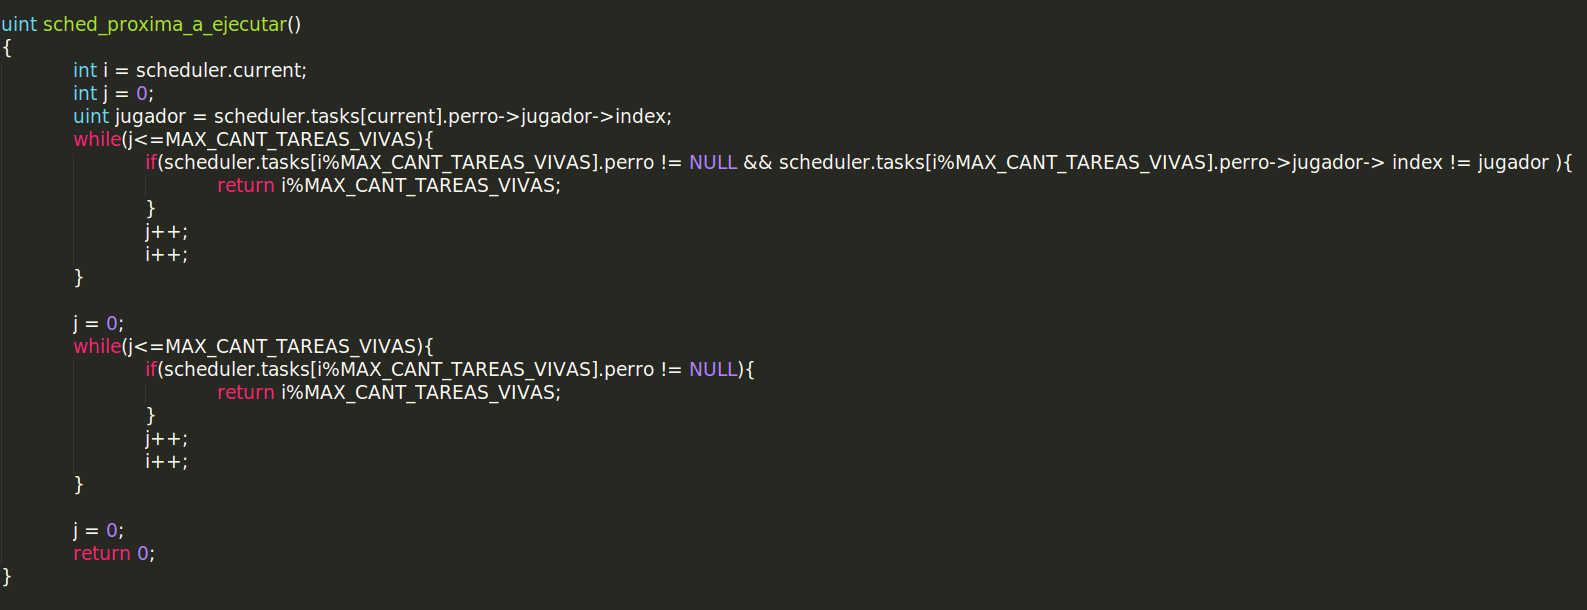
\includegraphics[width=\linewidth]{ejercicio7/proxeje.png}
\caption{{\small \textit{Funcion proxima tarea a ejecutar }}}
\endminipage
\end{center}
\end{figure}

\subsection{Ítem c):  Crear una función \textit{sched\_atender\_tick()}}

Esta función debería devolver la posicion de la \textit{GDT} de la proxima tarea, para eso utiliza la funcion del item anterior, además actualiza el int \textit{current} de la estructura del sheduler. 

\begin{figure}[H]
\begin{center}
\minipage{0.8\textwidth}
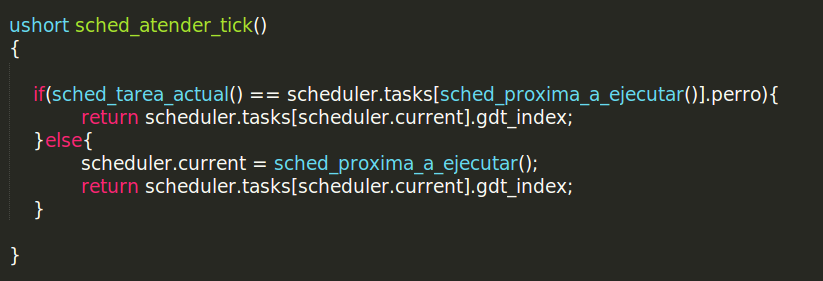
\includegraphics[width=\linewidth]{ejercicio7/atendtick.png}
\caption{{\small \textit{Funcion proxima tarea a ejecutar }}}
\endminipage
\end{center}
\end{figure}

\subsection{Ítem d):  Atender la interrupcion 0x46}

\subsection{Ítem e):  Realiza el intercabio e tareas}

El intercambio de tareas lo realizamos en cada interrupción del reloj, utilizando las funciones explicadas anteriormente. Para utilizarlas escribimos las siguientes lineas en la \textit{RAE} del reloj:

\begin{center}

    pushad \\    
    call fin\_intr\_pic1 \\
    call sched\_tarea\_actual \\
    push eax    \\
    call game\_atender\_tick \\           
    call sched\_atender\_tick \\

    str cx \\
    cmp ax,cx \\
    je .fin \\
    mov [selector], ax \\
    jmp selector:offset \\

    .fin: \\
     call screen\_actualizar\_reloj\_global \\    
    pop eax \\
    popad \\
    iret \\

\end{center}

Esta rutina pregunta por la poscicion de la \textit{GDT}  de la proxima tarea a ejecutar y si la proxima tarea a ejecutar es la misma que se esta ejecutando ahora no hace nada, sin embargo si es diferente realiza un \textit{jmp far} utilizando como selector la posicion en la \textit{GDT} correspondiente. De esta forma se  guarda la \textit{TSS} actual y se carga la nueva. 


